\chapter{結果と分析}
\label{chap:results}

\section{アニメーション生成結果}

\section{評価}

\subsection{実際の演奏シーンとの比較による評価}

\begin{figure}[t]
	\centering
	\subcaptionbox{\textgt{吹奏楽・オーケストラ経験者の回答}
		\label{fig:unity}}[0.75\linewidth]{
		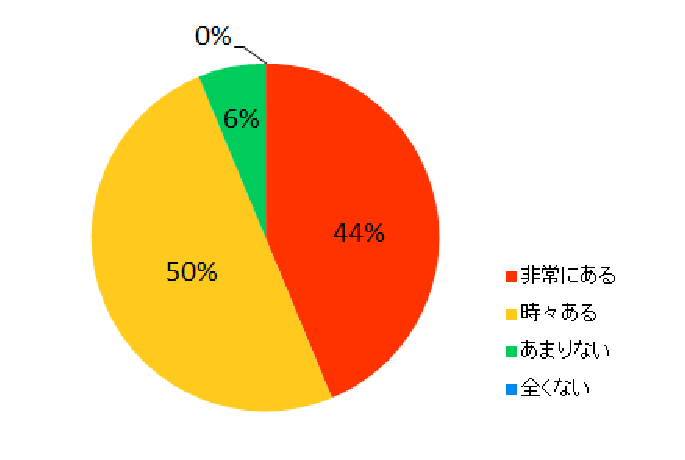
\includegraphics[height=7cm]{fig/chap1/Q1-1.eps}}
	\subcaptionbox{\textgt{吹奏楽・オーケストラ未経験者の回答}
		\label{fig:tp}}[0.6\linewidth]{
		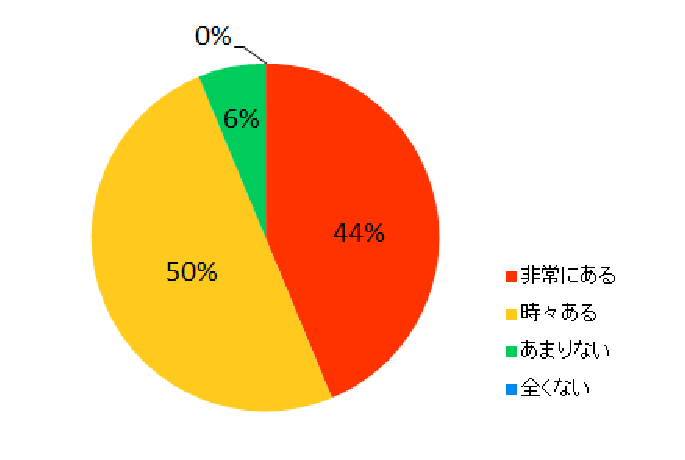
\includegraphics[height=5.5cm]{fig/chap1/Q1-2.eps}}
	\caption{演奏アニメーションが不自然であると感じることがあるかどうか}
	\label{fig:model}
\end{figure}

\subsection{既存のアニメーションとの比較による評価}

\subsection{アンサンブルアニメーションの評価}

\subsection{システムの有用性の予想}